\documentclass[11pt]{article}

% Language setting
\usepackage[turkish]{babel}
\usepackage{pythonhighlight}

\usepackage[a4paper,top=2cm,bottom=2cm,left=2cm,right=2cm,marginparwidth=2cm]{geometry}

% Useful packages
\usepackage{amsmath}
\usepackage{graphicx}
\usepackage[colorlinks=true, allcolors=blue]{hyperref}
\usepackage{verbatim}
\usepackage{fancyhdr} % for header and footer
\usepackage{titlesec}
\usepackage{parskip}

\setlength{\parindent}{0pt}

\titleformat{\subsection}[runin]{\bfseries}{\thesubsection}{1em}{}

\pagestyle{fancy} % activate the custom header/footer

% define the header/footer contents
\lhead{\small{23BLM-4014 Yapay Sinir Ağları Ara Sınav Soru ve Cevap Kağıdı}}
\rhead{\small{Dr. Ulya Bayram}}
\lfoot{}
\rfoot{}

% remove header/footer on first page
\fancypagestyle{firstpage}{
  \lhead{}
  \rhead{}
  \lfoot{}
  \rfoot{\thepage}
}
 

\title{Çanakkale Onsekiz Mart Üniversitesi, Mühendislik Fakültesi, Bilgisayar Mühendisliği Akademik Dönem 2022-2023\\
Ders: BLM-4014 Yapay Sinir Ağları/Bahar Dönemi\\ 
ARA SINAV SORU VE CEVAP KAĞIDI\\
Dersi Veren Öğretim Elemanı: Dr. Öğretim Üyesi Ulya Bayram}
\author{%
\begin{minipage}{\textwidth}
\raggedright
Öğrenci Adı Soyadı: Ömercan Yeşil\\ % Adınızı soyadınızı ve öğrenci numaranızı noktaların yerine yazın
Öğrenci No: 170401048
\end{minipage}%
}

\date{14 Nisan 2023}

\begin{document}
\maketitle

\vspace{-.5in}
\section*{Açıklamalar:}
\begin{itemize}
    \item Vizeyi çözüp, üzerinde aynı sorular, sizin cevaplar ve sonuçlar olan versiyonunu bu formatta PDF olarak, Teams üzerinden açtığım assignment kısmına yüklemeniz gerekiyor. Bu bahsi geçen PDF'i oluşturmak için LaTeX kullandıysanız, tex dosyasının da yer aldığı Github linkini de ödevin en başına (aşağı url olarak) eklerseniz bonus 5 Puan! (Tavsiye: Overleaf)
    \item Çözümlerde ya da çözümlerin kontrolünü yapmada internetten faydalanmak, ChatGPT gibi servisleri kullanmak serbest. Fakat, herkesin çözümü kendi emeğinden oluşmak zorunda. Çözümlerinizi, cevaplarınızı aşağıda belirttiğim tarih ve saate kadar kimseyle paylaşmayınız. 
    \item Kopyayı önlemek için Github repository'lerinizin hiçbirini \textbf{14 Nisan 2023, saat 15:00'a kadar halka açık (public) yapmayınız!} (Assignment son yükleme saati 13:00 ama internet bağlantısı sorunları olabilir diye en fazla ekstra 2 saat daha vaktiniz var. \textbf{Fakat 13:00 - 15:00 arası yüklemelerden -5 puan!}
    \item Ek puan almak için sağlayacağınız tüm Github repository'lerini \textbf{en geç 15 Nisan 2023 15:00'da halka açık (public) yapmış olun linklerden puan alabilmek için!}
    \item \textbf{14 Nisan 2023, saat 15:00'dan sonra gönderilen vizeler değerlendirilmeye alınmayacak, vize notu olarak 0 (sıfır) verilecektir!} Son anda internet bağlantısı gibi sebeplerden sıfır almayı önlemek için assignment kısmından ara ara çözümlerinizi yükleyebilirsiniz yedekleme için. Verilen son tarih/saatte (14 Nisan 2023, saat 15:00) sistemdeki en son yüklü PDF geçerli olacak.
    \item Çözümlerin ve kodların size ait ve özgün olup olmadığını kontrol eden bir algoritma kullanılacaktır. Kopya çektiği belirlenen vizeler otomatikman 0 (sıfır) alacaktır. Bu nedenle çözümlerinizi ve kodlarınızı yukarıda sağladığım gün ve saatlere kadar kimseyle paylaşmayınız.
    \item Bu vizeden alınabilecek en yüksek not 100'dür. Toplam aldığınız puan 100'ü geçerse, aldığınız not 100'e sabitlenecektir.
    \item LaTeX kullanarak PDF oluşturanlar öz geçmişlerine LaTeX bildiklerini de eklemeyi unutmasınlar :)
    \item Bu vizedeki soruların çözümleri ve tex dosyası için istediğiniz kadar sayıda Github repository'si oluşturabilirsiniz. Sadece yukarıda belirttiğim tarihlerde (14 Nisan 2023 saat 15:00 ile 15 Nisan 2023 saat 15:00 arasında) public yapmayı/halka açmayı ve Github profilinizi de öz geçmişinize eklemeyi unutmayın :)
    \item Bilgisayarınıza hiçbir program kurmadan, Overleaf, Google Colab, Kaggle gibi ortamlar üzerinden bu vizeyi tamamlamanız mümkün. İyi çalışmalar!!
\end{itemize}

(Ekstra 5 puan) \url{OdevinTexDosyasınınGithubLinkiniburayakoyun.com}

\newpage
\section{(Toplam 10 Puan) Hopfield Networks:}

\subsection{(2 Puan)} \textbf{ChatGPT’ye size Hopfield Network’ler ile ilgili detaylı bilgi vermesini isteyin. Sorduğunuz soruyu, ChatGPT'nin çıkartığı cevabı aşağı koyun. Bu cevapta anlamadığınız terimleri de ChatGPT’ye sorup, sorduğunuz soruları ve ChatGPT’nin verdiği cevapları da sırayla aşağı koyun.}

\textbf{Hopfield Network'lerle ilgili detaylı bilgi verir misin?}
Hopfield ağları, 1982'de John Hopfield tarafından tanımlanan, öz-düzenleyici yapısıyla dikkat çeken bir sinir ağı modelidir. Hopfield ağları, içinde belirli bir düzenin korunduğu bir dizi nöronun etkileşimini taklit eder.

Hopfield ağı, birçok nöronun etkileşimini simüle eder ve bu nöronlar birbirleriyle bağlıdır. Bu bağlantılar, ağın bir nöronun aktivasyon durumundan diğerininki hakkında bilgi edinebilmesini sağlar. Bu bağlantılar ağı simetrik yapar. Ağ, girdileri işleyebilir ve birçok durumda sonuçları hatırlayabilir.

Hopfield ağları, asıl olarak hatırlama ve optimizasyon problemlerinde kullanılır. Örneğin, bir Hopfield ağı, depolanan belirli desenleri hatırlayabilir ve bir desene yakın girdileri yakın bir depolanan desene eşleştirebilir. Ayrıca, Hopfield ağları, enerji fonksiyonları olarak adlandırılan matematiksel nesneleri optimize etmek için kullanılabilir. Bu fonksiyonlar, ağın belirli bir durumunda bulunan enerjiyi ölçer ve ağın enerjiyi en aza indirecek bir çözüm bulmasını sağlar.

Hopfield ağları, yapay sinir ağlarının tarihinde önemli bir yere sahip olmasına rağmen, bellek kapasiteleri sınırlıdır ve büyük ölçekli problemleri işlemek için yeterli olmayabilirler. Bununla birlikte, çeşitli uygulamalarda halen kullanılmaktadırlar ve birçok algoritma ve teknolojinin temelinde yer almaktadırlar.

\textbf{çalışma mantığı nasıldır?}
Hopfield ağları, nöronlar arasındaki bağlantıları kullanarak bir girdiyi işlerler ve sonucunda bir çıktı üretirler. Bu bağlantılar, ağın bir nöronun aktivasyon durumundan diğerininki hakkında bilgi edinebilmesini sağlar. Bağlantılar, ağı simetrik yapar, yani ağdaki her bir nöron, diğer nöronların aktivasyon durumu tarafından etkilenir ve aynı zamanda diğer nöronların aktivasyon durumunu etkiler.

Hopfield ağları, hatırlama ve optimizasyon problemlerini çözmek için kullanılırlar. Örneğin, bir Hopfield ağı, bir dizi girişi işleyerek depolanan bir desenle eşleşecek bir çıktı üretebilir. Bu desenler genellikle ağın belleğinde depolanır ve ağ, girdiyle benzer bir desen bulmak için bellekteki desenleri karşılaştırır.

Hopfield ağları, enerji fonksiyonları olarak adlandırılan matematiksel nesneleri optimize etmek için de kullanılabilirler. Bu fonksiyonlar, ağın belirli bir durumunda bulunan enerjiyi ölçer ve ağın enerjiyi en aza indirecek bir çözüm bulmasını sağlar.

Hopfield ağı, girdiyi nöronlar tarafından işler ve sonuçta bir çıktı üretir. Her nöron, bir aktivasyon seviyesine sahiptir ve bu seviye, diğer nöronların aktivasyon seviyeleri tarafından etkilenir. Ağ, belirli bir girdiyle eşleşen bir çıktıyı bulmak için nöronların aktivasyon seviyelerini birbirine yaklaştırmaya çalışır. Bu işlem, nöronların aktivasyon seviyelerinin ağın enerji fonksiyonunu minimize etmek için iteratif olarak güncellendiği bir optimizasyon işlemidir.

\textbf{bu ağın avantajları ve dezavantajları nelerdir?}
Hopfield ağlarının avantajları ve dezavantajları şunlardır:

Avantajları:

Hopfield ağları, özellikle hatırlama ve optimizasyon problemlerinde kullanıldığında yüksek doğruluk sağlarlar.
Ağın simetrik yapısı, bellek kapasitesini arttırır ve ağın daha fazla desenleri hatırlamasını sağlar.
Hopfield ağları, genellikle basit ve anlaşılır matematiksel yapısı sayesinde kolayca uygulanabilir ve programlanabilirler.
Ağın eğitimi, geleneksel yapay sinir ağlarında olduğu gibi, ağın kendi kendine öğrenmesi gerektiği için, daha fazla veri toplama veya etiketleme gibi önceden hazırlık gerektirmez.
Dezavantajları:

Hopfield ağlarının bellek kapasitesi sınırlıdır ve büyük ölçekli problemleri işlemek için yeterli olmayabilirler.
Ağın simetrik yapısı, girdilerin ağı etkileme şeklini sınırlar ve bu da ağın doğruluğunu düşürebilir.
Hopfield ağları, çoğunlukla basit problemlerle ilgilenirler ve daha karmaşık problemlerle başa çıkmak için özel olarak tasarlanmış diğer yapay sinir ağları gibi esnek değillerdir.
Ağın eğitimi, ağın enerji fonksiyonunu minimize etmek için iteratif olarak güncelleme işlemini gerektirir. Bu işlem, bazen yavaş olabilir ve ağın hızını düşürebilir.

\textbf{hopfield ağı günümüzde hangi alanlarda kullanılıyor?}
Hopfield ağları, bellek kapasiteleri sınırlı olduğu için günümüzde genellikle küçük ölçekli problemleri çözmek için kullanılır. Bu nedenle, Hopfield ağları, diğer yapay sinir ağı türleri ile birlikte kullanılarak daha büyük ve karmaşık problemleri çözmek için bir araç olarak kullanılabilirler. Hopfield ağları aşağıdaki alanlarda kullanılabilir:

Optimize Etme Problemleri: Hopfield ağları, optimize etme problemleri gibi problemleri çözmek için kullanılabilir. Örneğin, seyahat eden satıcı problemi gibi bir problemde, Hopfield ağı, en kısa rotayı bulmak için kullanılabilir.

Modelleme: Hopfield ağları, modelleme problemleri için de kullanılabilir. Örneğin, ağlar, hava durumu tahmini, finansal tahminler, ve biyolojik modeller gibi birçok alanda kullanılabilir.

Mühendislik: Hopfield ağları, mühendislik alanında da kullanılabilir. Örneğin, ağlar, tahmin, kontrol, ve denetim sistemleri gibi alanlarda kullanılabilir.

Görüntü İşleme: Hopfield ağları, görüntü işleme ve tanıma problemlerinde de kullanılabilir. Örneğin, ağlar, optik karakter tanıma (OCR) ve nesne tanıma gibi alanlarda kullanılabilir.

Hopfield ağları, bellek kapasiteleri sınırlı olsa da, basit yapısı, kolay programlanabilirliği ve farklı alanlarda kullanım imkanları nedeniyle hala birçok uygulama alanına sahiptir.
\subsection{(8 Puan)} \textbf{ChatGPT’nin açıklamalarından ne anladığınızı buraya kendi kelimelerinizle özetleyin. Örneğin ``Hopfield Network nedir? Ne işe yarar? Neden bilmemiz gerekir bunu? Gerçek hayatta kullanılıyor mu?'' gibi. Anlamadığınız kısımlar varsa ve ChatGPT’nin açıklamaları yeterli gelmezse internet dahil farklı kaynaklardan araştırıp, bilgilerin doğruluğunu sorgulamakta serbestsiniz. Konuyu doğru anlayıp anlamamanız puana etki edecektir. Kullandığınız kaynakları da belirtin!}

Hopfield ağı, tek bir katmana sahip bir sinir ağ modelidir. Bu model hatırlama ve optimizasyon problemlerinde kullanılır. Bu modelin bellek kapasitesi sınırlı olduğu için daha çok küçük ölçekli problemleri çözmek için kullanılır.  Eğitim aşamasında desenler hafızda depolanır, eğitim aşamasından sonra input olarak verilen bozuk desenin kısmi ipuçlarından ve önceden depolanmış desenlerden yararlanarak verilen bozuk deseni düzeltebilir. Hopfield ağları optimize etme problemleri, hava durumu tahminleri, finansal tahminleri, ve görüntü işlemede kullanılır.



\section{(Toplam 10 Puan) Boltzman Machine:}

\subsection{(2 Puan)} \textbf{ChatGPT’ye size Boltzman Machine ilgili detaylı bilgi vermesini isteyin. Sorduğunuz soruyu, ChatGPT'nin çıkartığı cevabı aşağı koyun. Bu cevapta anlamadığınız terimleri de ChatGPT’ye sorup, sorduğunuz soruları ve ChatGPT’nin verdiği cevapları da sırayla aşağı koyun.}

\textbf{Boltzman Machine ile ilgili detaylı bilgi verir misin?}
Boltzmann makineleri, yapay sinir ağları arasında bir tür olup, belirli bir problemin çözümü için kullanılabilirler. Boltzmann makineleri, biyolojik nöronların etkileşimlerini taklit eder ve bu nedenle sinir ağı modelleri arasında yaygın olarak kullanılırlar.

Bir Boltzmann makinesi, bir dizi gizli katmana ve görüntü katmanına sahiptir. Gizli katmanlar, ağın içindeki her bir nöronun etkinliğini temsil eder ve ağın öğrenme sırasında nasıl davrandığını belirler. Görüntü katmanı, ağa giriş verilerini temsil eder.

Bir Boltzmann makinesinin çalışması, her bir nöronun diğer nöronlarla bağlantılarının belirlenmesine dayanır. Bu bağlantılar ağırlıklar ile tanımlanır ve bu ağırlıklar, ağın belirli bir davranışını belirler. Ağırlıklar rastgele olarak başlatılır ve ardından ağ öğrenme algoritmasıyla güncellenir.

Öğrenme algoritması, ağın verileri işleyiş şeklini geliştirmek için ağırlıkları günceller. Bu ağırlıkların güncellenmesi, birbirleriyle etkileşimleri belirler. Ağırlıkların belirlenmesi, her bir nöronun diğer nöronlarla olan bağlantılarını belirler ve bu bağlantılar, ağın belirli bir davranışını belirler.

Boltzmann makineleri, çeşitli görevleri çözmek için kullanılabilirler. Örneğin, sayısal veri sıkıştırma, ses işleme, görüntü tanıma ve doğal dil işleme gibi alanlarda kullanılabilirler. Ayrıca, çeşitli optimizasyon problemlerinin çözümü için de kullanılabilirler.

Sonuç olarak, Boltzmann makineleri, sinir ağı modelleri arasında yaygın olarak kullanılan ve belirli problemlerin çözümü için kullanılabilen yapay sinir ağı türüdür.

\textbf{bozmalt makinelerinin kullanım alanları nelerdir?}
"Boltzmann" makineleri, yapay zeka alanında yaygın olarak kullanılan bir tür yapay sinir ağıdır. Boltzmann makineleri, çeşitli alanlarda kullanılabilirler ve bazı kullanım alanları şunlardır:

Veri Sıkıştırma: Boltzmann makineleri, sayısal verilerin sıkıştırılması için kullanılabilir. Bu teknoloji, yüksek boyutlu verilerin özetlenmesine ve daha sonra daha hızlı işlenmesine olanak tanır.

Doğal Dil İşleme: Boltzmann makineleri, doğal dil işleme uygulamalarında kullanılabilir. Bu teknoloji, metinleri analiz ederek, dil öğrenme modelleri oluşturarak ve konuşma tanıma gibi diğer dil işleme görevleri için kullanılabilir.

Görüntü Tanıma: Boltzmann makineleri, görüntü tanıma uygulamalarında kullanılabilir. Bu teknoloji, görüntülerdeki desenleri ve özellikleri öğrenerek, görüntüleri tanımak için kullanılabilir.

Otomatik Veri Sınıflandırma: Boltzmann makineleri, verileri otomatik olarak sınıflandırmak için kullanılabilir. Bu teknoloji, özellikle büyük veri kümelerinde etkili bir şekilde çalışır ve verileri gruplamak için kullanılabilir.

Öneri Sistemleri: Boltzmann makineleri, öneri sistemlerinin geliştirilmesinde kullanılabilir. Bu teknoloji, kullanıcı tercihlerini analiz ederek, onlara özelleştirilmiş öneriler yapmak için kullanılabilir.

Kimya ve Fizik: Boltzmann makineleri, kimya ve fizik alanlarında da kullanılabilir. Bu teknoloji, moleküler dinamikler ve fiziksel süreçler gibi karmaşık olayların modellenmesi için kullanılabilir.

Sonuç olarak, Boltzmann makineleri, birçok farklı alanda kullanılabilen çok yönlü bir teknolojidir ve her geçen gün yeni kullanım alanları keşfedilmektedir.

\textbf{hopfield ağı ile bir ilişkisi var mı?}
Evet, Boltzmann makineleri ve Hopfield ağları birbirleriyle yakından ilişkilidir. Hopfield ağları, Boltzmann makinelerinin özel bir türüdür. Bu iki model arasındaki fark, Hopfield ağlarının girdilerinin sabit olduğu, Boltzmann makinelerinde ise girdilerin değişebildiğidir.

Hopfield ağları, bir dizi bağlantılı nöronun etkileşimlerini simüle eden yapay sinir ağı modelleridir. Bu nöronlar, birbirleriyle etkileşim halindedir ve her biri, ağın toplam enerjisine katkıda bulunur. Ağın amacı, enerjinin en düşük seviyede kalması için nöronlar arasındaki bağlantıları yeniden yapılandırmaktır.

Boltzmann makineleri de Hopfield ağlarına benzer, ancak daha geniş bir uygulama yelpazesine sahiptirler. Boltzmann makineleri, birbirleriyle etkileşim halinde olan gizli ve görüntü katmanları içeren bir tür yapay sinir ağıdır. Bu katmanlar arasındaki etkileşimler, bir dizi bağlantılı nöronun enerjisinin hesaplanmasına dayanır.

Her iki model de öğrenme ve tahmin yapabilen yapay sinir ağı modelleridir ve geniş bir uygulama yelpazesine sahiptirler. Ancak, Boltzmann makineleri daha geniş bir uygulama yelpazesine sahip olduğu için, Hopfield ağlarına kıyasla daha yaygın olarak kullanılırlar.

\textbf{gizli katmanın ve görüntü katmanının görevi nedir?}
Gizli katmanlar ve görüntü katmanları, bir Boltzmann makinesinin temel yapı taşlarındandır ve her birinin farklı görevleri vardır.

Gizli katmanlar, Boltzmann makinesinin öğrenme sürecinde kullanılan bir dizi gizli nöron içerir. Bu katman, girdilerle doğrudan ilişkili olmayan ancak girdilerin öğrenilmesine yardımcı olan ara katmanlardır. Bu nöronlar, Boltzmann makinesinin öğrenmesi sırasında kullanılan sinir ağı yapısını oluşturur.

Gizli katmanlar, özellikle denetimsiz öğrenme teknikleri kullanılarak, veri kümesindeki örüntüleri tespit etmek ve verilerin doğrusal olmayan özelliklerini modellemek için kullanılır. Bu nedenle, gizli katmanlar, öğrenilen özelliklerin kodlanmasında ve veriler arasındaki bağlantıların modellenmesinde önemli bir rol oynar.

Görüntü katmanları ise, Boltzmann makinesinin girdi verilerini temsil ettiği katmandır. Bu katman, genellikle bir dizi piksel olarak temsil edilen görüntülerden oluşur. Bu görüntüler, öğrenme sırasında Boltzmann makinesine verilen ve öğrenilen özelliklerin modellenmesinde kullanılan girdi verileridir.

Görüntü katmanları, verilerin özelliklerini kodlamak ve bunları gizli katmanlara iletmek için kullanılır. Bu nedenle, Boltzmann makinesinin öğrenmesi sırasında, görüntü katmanlarından gelen veriler gizli katmanlardaki nöronlar tarafından işlenir ve öğrenilen özelliklerin kodlanması için kullanılır.

Sonuç olarak, gizli katmanlar ve görüntü katmanları, Boltzmann makinelerinin temel yapı taşlarıdır. Her birinin farklı görevleri vardır ve birlikte çalışarak, veriler arasındaki bağlantıları modelleyerek, özelliklerin öğrenilmesini sağlarlar.

\subsection{(8 Puan)} \textbf{ChatGPT’nin açıklamalarından ne anladığınızı buraya kendi kelimelerinizle özetleyin. Örneğin ``Boltzman Machine nedir? Ne işe yarar? Neden bilmemiz gerekir bunu? Gerçek hayatta kullanılıyor mu?'' gibi. Anlamadığınız kısımlar varsa ve ChatGPT’nin açıklamaları yeterli gelmezse internet dahil farklı kaynaklardan araştırıp, bilgilerin doğruluğunu sorgulamakta serbestsiniz. Konuyu doğru anlayıp anlamamanız puana etki edecektir. Kullandığınız kaynakları da belirtin!}

Boltzman mankinesi bir dizi gizli katmana ve görüntü katmanına sahiptir. Aynı katmandaki nöronlar birbirine bağlı değildir bundan dolayı katman içi iletişim yoktur. Gizli katman Boltzman makinesinin öğrenmesine yardımcı olan ara katmandır. Görüntü katmanı Boltzmann makinesinin girdi verilerini temsil ettiği katmandır. Boltzmann makinesinin öğrenmesi sırasında görüntü katmanından gelen veriler gizli katmanda işlenir. Bu şekilde katmanlar birlikte çalışarak, veriler arasındaki bağlantılar modellenerek makinenin öğrenmesi sağlanır.Boltzmann makinesi Hopfield ağlarının özel bir türüdür ancak Boltzmann makinelerinin daha geniş bir uygulama alanı vardır. Bu nedenle Boltzmann makineleri Hopfield ağlarına kıyasla daha yaygın olarak kullanılır. Boltzmann makineleri veri sıkıştırma, doğal dil işleme, görüntü tanıma gibi alanlarda kullanılıyor.

\section{(Toplam 10 Puan) Markov Assumption ve Markov Chain:}

\subsection{(2 Puan)} \textbf{ChatGPT’ye size Markov assumption ve Markov Chain ilgili detaylı bilgi vermesini isteyin. Sorduğunuz soruyu, ChatGPT'nin çıkartığı cevabı aşağı koyun. Bu cevapta anlamadığınız terimleri de ChatGPT’ye sorup, sorduğunuz soruları ve ChatGPT’nin verdiği cevapları da sırayla aşağı koyun.}

\textbf{Markov assumption ve Markov Chain ilgili detaylı bilgi verir misin}
Elbette, Markov assumption ve Markov Chain kavramları oldukça önemlidir ve çeşitli alanlarda yaygın olarak kullanılmaktadır.

Markov assumption, bir sistemin gelecekteki davranışının yalnızca mevcut durumuna bağlı olduğunu varsayar. Başka bir deyişle, gelecekteki durumlar sadece şu anda mevcut olan durumdan etkilenir ve geçmiş durumlar gelecekteki davranışı etkilemez. Bu varsayım, özellikle zaman serileri analizinde kullanılmaktadır ve Markov Zincirleri'nin temelini oluşturur.

Markov Zinciri ise, bir dizi rastgele değişkenin, Markov assumption'a uygun bir şekilde, yalnızca mevcut durumuna bağlı olarak zaman içindeki durumlarını tanımlayan matematiksel bir modeldir. Markov Zinciri, diskret ve sürekli zamanlı olabilir ve birçok alanda kullanılabilir, örneğin mühendislik, finans, biyoloji, bilgisayar bilimi ve fizik gibi alanlarda. Markov Zinciri'nin temel özellikleri arasında geçiş olasılıkları, olasılık dağılımları, denge durumu ve kararlılık gibi özellikler yer almaktadır.

Markov Zinciri'nin kullanımı, özellikle öngörü ve tahmin yapma gibi konularda oldukça faydalıdır. Örneğin, bir finansal piyasanın gelecekteki fiyat hareketlerini tahmin etmek için, Markov Zinciri kullanılabilir. Ayrıca, doğal dil işleme ve konuşma sentezi gibi alanlarda da kullanılabilir.

Sonuç olarak, Markov Zinciri ve Markov assumption, sistemlerin gelecekteki davranışlarını anlamak ve öngörmek için kullanılan güçlü matematiksel araçlardır ve birçok alanda yaygın olarak kullanılmaktadır.

\textbf{Markov zincirinin kullanım alanları nedir?}
Markov Zinciri'nin kullanım alanları oldukça geniş kapsamlıdır. İşte bazı örnekler:

Finansal piyasa analizi: Markov Zincirleri, hisse senetleri, döviz kurları ve emtia fiyatları gibi finansal varlıkların fiyat hareketlerini tahmin etmek için kullanılır.

Doğal Dil İşleme: Markov Zincirleri, kelime tahmin etmek veya metinleri sınıflandırmak gibi doğal dil işleme uygulamalarında kullanılabilir.

Robotik ve Otomasyon: Markov Zincirleri, robotların hareketlerini planlamak veya bir robotik sistemdeki sensör verilerini analiz etmek için kullanılabilir.

Biyoinformatik: Markov Zincirleri, DNA dizilerini analiz etmek veya protein yapıları gibi biyomoleküllerin dinamiklerini modellemek için kullanılabilir.

Mühendislik: Markov Zincirleri, trafik akışı, ağ trafiği veya enerji yönetimi gibi alanlarda kullanılabilir.

İstatistiksel Fizik: Markov Zincirleri, birçok parçacık sistemlerinin dinamiklerini modellemek için kullanılır.

Makine Öğrenimi: Markov Zincirleri, öğrenme algoritmalarının bir parçası olarak kullanılabilir.

Epidemiyoloji: Markov Zincirleri, hastalık yayılımını modellemek veya epidemiyolojik verileri analiz etmek için kullanılabilir.

Sinyal İşleme: Markov Zincirleri, sinyallerin öngörülmesi veya sinyal sınıflandırması gibi uygulamalarda kullanılabilir.

Bu sadece Markov Zincirlerinin kullanılabileceği birkaç örnek. Bu yöntem, daha birçok farklı alanda ve uygulamada kullanılmaktadır.

\textbf{Markov zincirinin çalışma mantığı nedir?}
Markov Zincirleri, bir sistemin gelecekteki durumunu sadece şu anki durumu ile tanımlayan bir matematiksel modeldir. Bu tanımlama, Markov Zinciri'nin çalışma mantığının temelini oluşturur. Bir Markov Zinciri, bir dizi rastgele değişkenin durumlarından oluşur ve bu durumlar birbirleriyle ilişkilidir.

Bir Markov Zinciri'nin çalışma mantığı şöyledir:

Durumlar: Markov Zinciri, birbirine bağlı durumlardan oluşur. Her durum, sistemin bulunduğu belirli bir durumu temsil eder.

Geçiş Olasılıkları: Markov Zinciri'ndeki her bir durum, diğer durumlara geçiş yapabilen belirli bir olasılığa sahiptir. Bu olasılıklar, her bir durumdan diğer durumlara geçişler için tanımlanır ve geçiş matrisi adı verilen bir matriste saklanır.

Markov Property: Markov Zincirleri, Markov Property olarak bilinen bir özellikle tanımlanır. Bu özellik, sistemin gelecekteki durumunun yalnızca şu anki durumuna bağlı olduğunu belirtir. Başka bir deyişle, geçmiş durumlar, sistemin gelecekteki davranışını etkilemez.

Denge Durumu: Markov Zincirleri, denge durumunda bulunabilir. Denge durumu, sistemin zamanla sabit hale gelmesi anlamına gelir. Bu durumda, herhangi bir durumda kalma olasılığı, sistemin durumundan bağımsızdır ve zincirin uzun vadeli davranışını belirler.

Markov Zincirleri, genellikle bir başlangıç durumu ve bir hedef durumu belirtilerek tanımlanır. Zincirin geçtiği durumlar, zaman içinde rastgele seçilir ve zincirin davranışı hakkında bilgi sağlar. Zincirin uzun vadeli davranışı, zincirin geçiş matrisi ve başlangıç durumu ile birlikte belirlenir.

Sonuç olarak, Markov Zincirleri, sistemin gelecekteki davranışını yalnızca şu anki durumuna bağlı olarak modelleyen bir matematiksel modeldir. Bu model, birçok alanda kullanılan birçok uygulama sunar.

\subsection{(8 Puan)} \textbf{ChatGPT’nin açıklamalarından ne anladığınızı buraya kendi kelimelerinizle özetleyin. Örneğin ``Markov assumption ve Markov Chain nedir? Ne işe yarar? Neden bilmemiz gerekir bunu? Gerçek hayatta kullanılıyor mu?'' gibi. Anlamadığınız kısımlar varsa ve ChatGPT’nin açıklamaları yeterli gelmezse internet dahil farklı kaynaklardan araştırıp, bilgilerin doğruluğunu sorgulamakta serbestsiniz. Konuyu doğru anlayıp anlamamanız puana etki edecektir. Kullandığınız kaynakları da belirtin!}

Markov Assumption bir sistemin gelecekteki davranışın sadece bulunduğu duruma bağlı olduğunu söyler. Gelecekteki durumlar yalnızca mevcut durumdan etkilenip geçmişten etkilenmezler. Bir başka deyişle, mevcut durumdaki veriler, sürecin gelecekteki evrimini etkileyebilecek tüm bilgiyi kapsar. Markov Zinciri ise Markov Assumption'a dayalı oluşturulmuş bir süreçtir. Markov Zinciri ve Markov Assumption sistemlerin gelecekteki davranışlarını ön görmeyi sağlar.  Markov zincirleri, birçok gerçek dünya sürecini modellemek için tasarlanabildikleri için çeşitli durumlarda kullanılır.

\section{(Toplam 20 Puan) Feed Forward:}
 
\begin{itemize}
    \item Forward propagation için, input olarak şu X matrisini verin (tensöre çevirmeyi unutmayın):\\
    $X = \begin{bmatrix}
        1 & 2 & 3\\
        4 & 5 & 6
        \end{bmatrix}$
    Satırlar veriler (sample'lar), kolonlar öznitelikler (feature'lar).
    \item Bir adet hidden layer olsun ve içinde tanh aktivasyon fonksiyonu olsun
    \item Hidden layer'da 50 nöron olsun
    \item Bir adet output layer olsun, tek nöronu olsun ve içinde sigmoid aktivasyon fonksiyonu olsun
\end{itemize}

Tanh fonksiyonu:\\
$f(x) = \frac{exp(x) - exp(-x)}{exp(x) + exp(-x)}$
\vspace{.2in}

Sigmoid fonksiyonu:\\
$f(x) = \frac{1}{1 + exp(-x)}$

\vspace{.2in}
 \textbf{Pytorch kütüphanesi ile, ama kütüphanenin hazır aktivasyon fonksiyonlarını kullanmadan, formülünü verdiğim iki aktivasyon fonksiyonunun kodunu ikinci haftada yaptığımız gibi kendiniz yazarak bu yapay sinir ağını oluşturun ve aşağıdaki üç soruya cevap verin.}
 
\subsection{(10 Puan)} \textbf{Yukarıdaki yapay sinir ağını çalıştırmadan önce pytorch için Seed değerini 1 olarak set edin, kodu aşağıdaki kod bloğuna ve altına da sonucu yapıştırın:}

% Latex'de kod koyabilirsiniz python formatında. Aşağıdaki örnekleri silip içine kendi kodunuzu koyun
\begin{python}
import torch
data = [[1.0,2.0,3.0],[4.0,5.0,6.0]]
x = torch.tensor(data).reshape(-1,2)

torch.manual_seed(1)

hidden_size = 50

w1 = torch.randn(hidden_size, 3)

output_size = 1

w2 = torch.randn(output_size, hidden_size)

b1 = torch.randn(hidden_size, 2)

b2 = torch.randn(output_size,2)

def sigmoid_activation(x):

  return 1 / (1 + torch.exp(-x))

def tanh(x):
  return (torch.exp(x) - torch.exp(-x)) / (torch.exp(x) + torch.exp(-x))

hidden_layer = tanh(torch.matmul(w1, x) + b1)

output_layer = sigmoid_activation(torch.matmul(w2, hidden_layer) + b2)

print(output_layer)
\end{python}

tensor([[0.0006, 0.0023]])

\subsection{(5 Puan)} \textbf{Yukarıdaki yapay sinir ağını çalıştırmadan önce Seed değerini öğrenci numaranız olarak değiştirip, kodu aşağıdaki kod bloğuna ve altına da sonucu yapıştırın:}

\begin{python}
import torch

data = [[1.0,2.0,3.0],[4.0,5.0,6.0]]
x = torch.tensor(data).reshape(-1,2)

torch.manual_seed(170401048)

hidden_size = 50

w1 = torch.randn(hidden_size, 3)

output_size = 1

w2 = torch.randn(output_size, hidden_size)

b1 = torch.randn(hidden_size, 2)

b2 = torch.randn(output_size,2)

def sigmoid_activation(x):

  return 1 / (1 + torch.exp(-x))

def tanh(x):
  return (torch.exp(x) - torch.exp(-x)) / (torch.exp(x) + torch.exp(-x))

hidden_layer = tanh(torch.matmul(w1, x) + b1)

output_layer = sigmoid_activation(torch.matmul(w2, hidden_layer) + b2)

print(output_layer)
\end{python}

tensor([[1.0000, 0.7556]])

\subsection{(5 Puan)} \textbf{Kodlarınızın ve sonuçlarınızın olduğu jupyter notebook'un Github repository'sindeki linkini aşağıdaki url kısmının içine yapıştırın. İlk sayfada belirttiğim gün ve saate kadar halka açık (public) olmasın:}
% size ait Github olmak zorunda, bu vize için ayrı bir github repository'si açıp notebook'u onun içine koyun. Kendine ait olmayıp da arkadaşının notebook'unun linkini paylaşanlar 0 alacak.

\url{https://github.com/yesilc/forward-propagation-nn/blob/main/untitled0.ipynb}

\section{(Toplam 40 Puan) Multilayer Perceptron (MLP):} 
\textbf{Bu bölümdeki sorularda benim vize ile beraber paylaştığım Prensesi İyileştir (Cure The Princess) Veri Seti parçaları kullanılacak. Hikaye şöyle (soruyu çözmek için hikaye kısmını okumak zorunda değilsiniz):} 

``Bir zamanlar, çok uzaklarda bir ülkede, ağır bir hastalığa yakalanmış bir prenses yaşarmış. Ülkenin kralı ve kraliçesi onu iyileştirmek için ellerinden gelen her şeyi yapmışlar, ancak denedikleri hiçbir çare işe yaramamış.

Yerel bir grup köylü, herhangi bir hastalığı iyileştirmek için gücü olduğu söylenen bir dizi sihirli malzemeden bahsederek kral ve kraliçeye yaklaşmış. Ancak, köylüler kral ile kraliçeyi, bu malzemelerin etkilerinin patlayıcı olabileceği ve son zamanlarda yaşanan kuraklıklar nedeniyle bu malzemelerden sadece birkaçının herhangi bir zamanda bulunabileceği konusunda uyarmışlar. Ayrıca, sadece deneyimli bir simyacı bu özelliklere sahip patlayıcı ve az bulunan malzemelerin belirli bir kombinasyonunun prensesi iyileştireceğini belirleyebilecekmiş.

Kral ve kraliçe kızlarını kurtarmak için umutsuzlar, bu yüzden ülkedeki en iyi simyacıyı bulmak için yola çıkmışlar. Dağları tepeleri aşmışlar ve nihayet "Yapay Sinir Ağları Uzmanı" olarak bilinen yeni bir sihirli sanatın ustası olarak ün yapmış bir simyacı bulmuşlar.

Simyacı önce köylülerin iddialarını ve her bir malzemenin alınan miktarlarını, ayrıca iyileşmeye yol açıp açmadığını incelemiş. Simyacı biliyormuş ki bu prensesi iyileştirmek için tek bir şansı varmış ve bunu doğru yapmak zorundaymış. (Original source: \url{https://www.kaggle.com/datasets/unmoved/cure-the-princess})

(Buradan itibaren ChatGPT ve Dr. Ulya Bayram'a ait hikayenin devamı)

Simyacı, büyülü bileşenlerin farklı kombinasyonlarını analiz etmek ve denemek için günler harcamış. Sonunda birkaç denemenin ardından prensesi iyileştirecek çeşitli karışım kombinasyonları bulmuş ve bunları bir veri setinde toplamış. Daha sonra bu veri setini eğitim, validasyon ve test setleri olarak üç parçaya ayırmış ve bunun üzerinde bir yapay sinir ağı eğiterek kendi yöntemi ile prensesi iyileştirme ihtimalini hesaplamış ve ikna olunca kral ve kraliçeye haber vermiş. Heyecanlı ve umutlu olan kral ve kraliçe, simyacının prensese hazırladığı ilacı vermesine izin vermiş ve ilaç işe yaramış ve prenses hastalığından kurtulmuş.

Kral ve kraliçe, kızlarının hayatını kurtardığı için simyacıya krallıkta kalması ve çalışmalarına devam etmesi için büyük bir araştırma bütçesi ve çok sayıda GPU'su olan bir server vermiş. İyileşen prenses de kendisini iyileştiren yöntemleri öğrenmeye merak salıp, krallıktaki üniversitenin bilgisayar mühendisliği bölümüne girmiş ve mezun olur olmaz da simyacının yanında, onun araştırma grubunda çalışmaya başlamış. Uzun yıllar birlikte krallıktaki insanlara, hayvanlara ve doğaya faydalı olacak yazılımlar geliştirmişler, ve simyacı emekli olduğunda prenses hem araştırma grubunun hem de krallığın lideri olarak hayatına devam etmiş.

Prenses, kendisini iyileştiren veri setini de, gelecekte onların izinden gidecek bilgisayar mühendisi prensler ve prensesler başkalarına faydalı olabilecek yapay sinir ağları oluşturmayı öğrensinler diye halka açmış ve sınavlarda kullanılmasını salık vermiş.''

\textbf{İki hidden layer'lı bir Multilayer Perceptron (MLP) oluşturun beşinci ve altıncı haftalarda yaptığımız gibi. Hazır aktivasyon fonksiyonlarını kullanmak serbest. İlk hidden layer'da 100, ikinci hidden layer'da 50 nöron olsun. Hidden layer'larda ReLU, output layer'da sigmoid aktivasyonu olsun.}

\textbf{Output layer'da kaç nöron olacağını veri setinden bakıp bulacaksınız. Elbette bu veriye uygun Cross Entropy loss yöntemini uygulayacaksınız. Optimizasyon için Stochastic Gradient Descent yeterli. Epoch sayınızı ve learning rate'i validasyon seti üzerinde denemeler yaparak (loss'lara overfit var mı diye bakarak) kendiniz belirleyeceksiniz. Batch size'ı 16 seçebilirsiniz.}

\subsection{(10 Puan)} \textbf{Bu MLP'nin pytorch ile yazılmış class'ının kodunu aşağı kod bloğuna yapıştırın:}

\begin{python}
class MLP(nn.Module):
    def __init__(self, input_size, hidden_size1, hidden_size2, output_size):
        super(MLP, self).__init__()
        self.hidden_layer1 = nn.Linear(input_size, hidden_size1)
        self.hidden_layer2 = nn.Linear(hidden_size1, hidden_size2)
        self.output_layer = nn.Linear(hidden_size2, output_size)
        self.relu = nn.ReLU()
        self.sigmoid = nn.Sigmoid()

    def forward(self, x):
        hidden1_res = self.relu(self.hidden_layer1(x))
        hidden2_res = self.relu(self.hidden_layer2(hidden1_res))
        out = self.sigmoid(self.output_layer(hidden2_res))
        return out
\end{python}

\subsection{(10 Puan)} \textbf{SEED=öğrenci numaranız set ettikten sonra altıncı haftada yazdığımız gibi training batch'lerinden eğitim loss'ları, validation batch'lerinden validasyon loss değerlerini hesaplayan kodu aşağıdaki kod bloğuna yapıştırın ve çıkan figürü de alta ekleyin.}

\begin{python}
import seaborn as sns
from matplotlib import pyplot as plt

learning_rate = 0.03
num_epochs = 80
input_size = a.size(1)

mlp = MLP(a.size(1)-1, hidden_size1=100, hidden_size2=50, output_size=1)
loss_fn = nn.BCELoss()
optimizer = torch.optim.SGD(mlp.parameters(), lr=learning_rate)


for epoch in range(num_epochs):

    # training loop
    train_loss = 0.0
    train_count = 0.0
    for i, data in enumerate(train_dataloader):
         inputs = data[:, :-1]
         labels = data[:, -1]

         optimizer.zero_grad()
         outputs = mlp(inputs)
         labels = labels.unsqueeze(1)
         loss = loss_fn(outputs, labels)
         loss.backward()
         optimizer.step()

         train_loss += loss.item()
         train_count += 1.0
       

    # validation loop
    val_loss = 0.0
    val_count = 0.0
    for j, val_data in enumerate(val_dataloader):
        val_inputs = val_data[:, :-1]
        val_labels = val_data[:, -1]

        with torch.no_grad():
            mlp.eval()
            val_outputs = mlp(val_inputs)
            val_labels = val_labels.unsqueeze(1)
            val_loss += loss_fn(val_outputs, val_labels).item()
            val_count += 1.0

    mlp.train()
    print("Epoch", epoch, "Training loss", train_loss/train_count, "Validation loss", val_loss/val_count)


sns.set_style("darkgrid")
plt.plot(list_train_loss, label="Training loss")
plt.plot(list_val_loss, label="Validation loss")
plt.xlabel("Epoch")
plt.ylabel("Loss")
plt.legend()
plt.show()
print('Finished Training')
\end{python}

% Figure aşağıda comment içindeki kısımdaki gibi eklenir.

\begin{figure}[ht!]
    \centering
    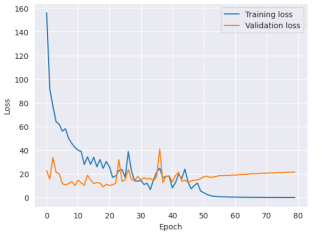
\includegraphics[width=0.75\textwidth]{epoch1.png}
    \caption{Loss değerlerinin her epoch'taki değişimi}
    \label{fig:my_pic}
\end{figure}


\subsection{(10 Puan)} \textbf{SEED=öğrenci numaranız set ettikten sonra altıncı haftada ödev olarak verdiğim gibi earlystopping'deki en iyi modeli kullanarak, Prensesi İyileştir test setinden accuracy, F1, precision ve recall değerlerini hesaplayan kodu yazın ve sonucu da aşağı yapıştırın. \%80'den fazla başarı bekliyorum test setinden. Daha düşükse başarı oranınız, nerede hata yaptığınızı bulmaya çalışın. \%90'dan fazla başarı almak mümkün (ben denedim).}

\begin{python}
from sklearn.metrics import accuracy_score, f1_score, precision_score, recall_score

# Kaydedilmiş en iyi modeli yükleme
model = MLP(a.size(1)-1, hidden_size1=100, hidden_size2=50, output_size=1)
model.load_state_dict(torch.load("checkpoint.pt"))

# Test dataloader'ından tahminleri alma
y_true = []
y_pred = []
model.eval()
with torch.no_grad():
    for data in test_dataloader:
        inputs = data[:, :-1]
        labels = data[:, -1]

        outputs = model(inputs)
        outputs = (outputs > 0.5).int() # Tahminlerimizi 0.5 sınırına göre binary formata dönüştürüyoruz

        y_true += labels.tolist()
        y_pred += outputs.tolist()

# Accuracy, F1, precision ve recall değerlerini hesaplama
accuracy = accuracy_score(y_true, y_pred)
f1 = f1_score(y_true, y_pred)
precision = precision_score(y_true, y_pred)
recall = recall_score(y_true, y_pred)

print("Accuracy:", accuracy)
print("F1 score:", f1)
print("Precision:", precision)
print("Recall:", recall)
\end{python}

Accuracy: 0.9481865284974094
F1 score: 0.9483204134366925
Precision: 0.9507772020725389
Recall: 0.9458762886597938


\subsection{(5 Puan)} \textbf{Tüm kodların CPU'da çalışması ne kadar sürüyor hesaplayın. Sonra to device yöntemini kullanarak modeli ve verileri GPU'ya atıp kodu bir de böyle çalıştırın ve ne kadar sürdüğünü hesaplayın. Süreleri aşağıdaki tabloya koyun. GPU için Google Colab ya da Kaggle'ı kullanabilirsiniz, iki ortam da her hafta saatlerce GPU hakkı veriyor.}

\begin{table}[ht!]
    \centering
    \caption{Buraya bir açıklama yazın}
    \begin{tabular}{c|c}
        Ortam & Süre (saniye) \\\hline
        CPU & 13 s \\
        GPU & 14.8 s\\
    \end{tabular}
    \label{tab:my_table}
\end{table}

\subsection{(3 Puan)} \textbf{Modelin eğitim setine overfit etmesi için elinizden geldiği kadar kodu gereken şekilde değiştirin, validasyon loss'unun açıkça yükselmeye başladığı, training ve validation loss'ları içeren figürü aşağı koyun ve overfit için yaptığınız değişiklikleri aşağı yazın. Overfit, tam bir çanak gibi olmalı ve yükselmeli. Ona göre parametrelerle oynayın.}

epoch sayısını ve learning rate'i arttırarak modelin overfit etmesini sağladım.

% Figür aşağı

\begin{figure}[ht!]
    \centering
    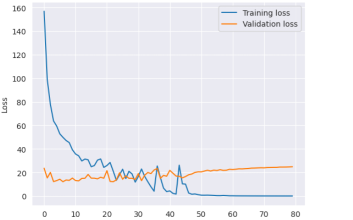
\includegraphics[width=0.75\textwidth]{epoch2.png}
    \caption{Overfit durumu}
    \label{fig:my_pic}
\end{figure}


\subsection{(2 Puan)} \textbf{Beşinci soruya ait tüm kodların ve cevapların olduğu jupyter notebook'un Github linkini aşağıdaki url'e koyun.}

\url{https://github.com/yesilc/cure-the-princess-nn-torch/blob/main/Untitled2.ipynb}

\section{(Toplam 10 Puan)} \textbf{Bir önceki sorudaki Prensesi İyileştir problemindeki yapay sinir ağınıza seçtiğiniz herhangi iki farklı regülarizasyon yöntemi ekleyin ve aşağıdaki soruları cevaplayın.} 

\subsection{(2 puan)} \textbf{Kodlarda regülarizasyon eklediğiniz kısımları aşağı koyun:} 

\begin{python}
import torch.nn as nn
class MLP(nn.Module):
    def __init__(self, input_size, hidden_size1, hidden_size2, output_size, dropout_rate):
        super(MLP, self).__init__()
        self.hidden_layer1 = nn.Linear(input_size, hidden_size1)
        self.dropout1 = nn.Dropout(p=dropout_rate)
        self.hidden_layer2 = nn.Linear(hidden_size1, hidden_size2)
        self.dropout2 = nn.Dropout(p=dropout_rate)
        self.output_layer = nn.Linear(hidden_size2, output_size)
        self.relu = nn.ReLU()
        self.sigmoid = nn.Sigmoid()

    def forward(self, x):
        hidden1_res = self.relu(self.hidden_layer1(x))
        hidden1_dropout = self.dropout1(hidden1_res)
        hidden2_res = self.relu(self.hidden_layer2(hidden1_dropout))
        hidden2_dropout = self.dropout2(hidden2_res)
        out = self.sigmoid(self.output_layer(hidden2_dropout))
        return out


optimizer = torch.optim.SGD(mlp.parameters(), lr=learning_rate, weight_decay=0.001)
\end{python}

\subsection{(2 puan)} \textbf{Test setinden yeni accuracy, F1, precision ve recall değerlerini hesaplayıp aşağı koyun:}

Accuracy: 0.9365284974093264
F1 score: 0.934228187919463
Precision: 0.9747899159663865
Recall: 0.8969072164948454


\subsection{(5 puan)} \textbf{Regülarizasyon yöntemi seçimlerinizin sebeplerini ve sonuçlara etkisini yorumlayın:}

Dropout ile rastgele şekilde nöronların söndürülmesi, tüm nöronların weight değerlerinin senkronije şekilde optimize etmesini engeller yani nöronlar arasındaki ilişkiyi keser. Bu şekilde overfitting azaltılır.
Weight decay ise ağın ağırlıklarının büyüklüğünü azaltarak overfitting sorununu azaltır. Bu iki regularizasyon yöntemini kodda uyguladığımda aynı epoch ve aynı learning rate değerleri ile daha önce artan validation loss değri bu sefer artış göstermedi aksine azaldı.

\subsection{(1 puan)} \textbf{Sonucun github linkini  aşağıya koyun:}

\url{https://github.com/yesilc/cure-the-princess-nn-torch/blob/main/Untitled2_ipynb_adl%C4%B1_not_defterinin_kopyas%C4%B1.ipynb}

\end{document}